\section{Database}

Il diagramma E-R (entità-relazione) riportato a seguito illustra la struttura e le relazioni all'interno del database.

\begin{figure}[H]
    \centering
    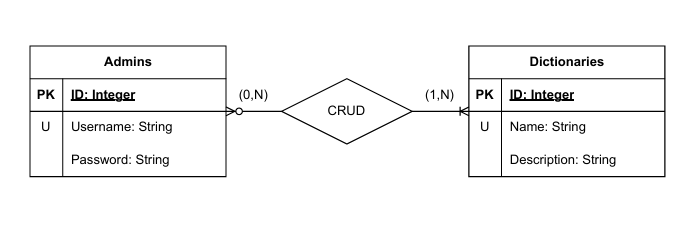
\includegraphics[width=0.95\textwidth]{assets/Database/DiagrammiDB.png}
    \caption{Diagramma E-R dell'interazione tra Admins (Tecnici) e \glossario{dizionari dati} per le operazioni \glossario{CRUD}}
\end{figure}

\subsection{Descrizione}
Il diagramma utilizza la notazione standard per le descrizioni dei database relazionali, dove le entità sono rapprentate dai rettagoli mentre le relazioni sono le linee che collegano le entità. Le sigle indicate rapprentano le indicazioni per le chiavi primarie (PK) e gli attributi unici (U) all'interno delle entità. Le linee terminano con dei simboli che ne indicano la cardinalità. Le tabelle sono inoltre collegate ad un rombo che rappresenta la relazione tra di esse: questa relazione non è una tabella, ma serve solo a scopo illustrativo.

\subsubsection{Tabella Admins}
La tabella \textbf{Admins} contiene i seguenti campi:
\begin{itemize}
    \item \textbf{PK ID}: un identificatore unico per ogni amministratore, di tipo integer;
    \item \textbf{U Username}: il nome utente dell'amministratore, di tipo string;
    \item \textbf{Password}: la password dell'amministratore, di tipo string.
\end{itemize}
Ogni entry della tabella descrive un Admin, cioè un Tecnico che può eseguire operaizoni CRUD sui dizionari dati.

\subsubsection{Tabella Dictionaries}
La tabella \textbf{Dictionaries} include i seguenti campi:
\begin{itemize}
    \item \textbf{PK ID}: un identificatore unico per ogni dizionario, di tipo integer;
    \item \textbf{U Name}: il nome del dizionario, di tipo string;
    \item \textbf{Description}: una descrizione del dizionario, di tipo string.
\end{itemize}

\subsubsection{Relazione}
Il diagramma mostra anche le operazioni CRUD (Create, Read, Update, Delete) che possono essere eseguite su queste tabelle. 

\begin{itemize}
    \item La relazione \textbf{0-N} : un admin può operare da 0 a N dizionari;
    \item La notazione \textbf{1-N} : su un dizonario possono operare da 1 a N admin.
\end{itemize}